\documentclass{standalone}
\usepackage{tikz}
\usepackage{ctex,siunitx,ninecolors}
\setCJKmainfont{Noto Serif CJK SC}
\usepackage{tkz-euclide}
\usepackage{amsmath}
\usepackage{wasysym}
\usetikzlibrary{patterns, calc}
\usetikzlibrary {decorations.pathmorphing, decorations.pathreplacing, decorations.shapes,}
\begin{document}
\small
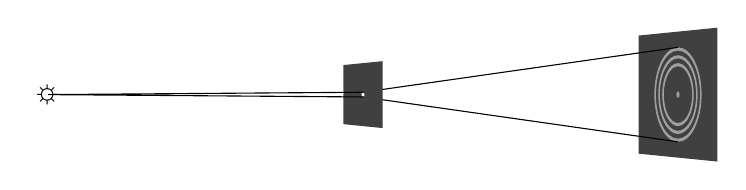
\begin{tikzpicture}[>=latex,scale=1.0]
  \node at (0,0){\sun};
  \fill[darkgray](7.5,0.75)--(7.5,-0.75)--(8.5,-0.85)--(8.5,0.85)--cycle;
  \fill[white,opacity=0.5,even odd rule](8,0)ellipse(0.3 and 0.6)(8,0)ellipse(0.28 and 0.56)(8,0)ellipse(0.25 and 0.5)(8,0)ellipse(0.23 and 0.46)(8,0)ellipse(0.20 and 0.4)(8,0)ellipse(0.18 and 0.36)(8,0)ellipse(0.02 and 0.04);
  \draw(8,-0.6)--(4,-0.03)(4,0.03)--(8,0.6);
  \fill[darkgray,even odd rule](3.75,0.375)--(3.75,-0.375)--(4.25,-0.425)--(4.25,0.425)--cycle (4,0)ellipse( 0.02 and 0.03);
  \draw(4,-0.03)--(0,0)--(4,0.03);
\end{tikzpicture}
\end{document}